% ==============================================================================
% Results and Discussion: Sorghum Stem Volume GWAS Analysis
% For Bioinformatics Journal
% ==============================================================================

\documentclass[11pt]{article}
\usepackage[utf8]{inputenc}
\usepackage{graphicx}
\usepackage{booktabs}
\usepackage{longtable}
\usepackage{amsmath}
\usepackage{hyperref}
\usepackage[margin=1in]{geometry}
\usepackage{caption}
\usepackage{multirow}
\usepackage{array}
\usepackage{xcolor}

\begin{document}

% ==============================================================================
\section{Results}
% ==============================================================================

\subsection{Genome-Wide Association Analysis Identifies Significant Loci for Stem Volume in Sorghum}

To identify genetic variants associated with stem volume in sorghum, we performed genome-wide association studies (GWAS) using a diverse sorghum association panel (SAP). The GWAS analysis identified multiple significant associations across the genome, with a pronounced signal on chromosome 9 (Figure~\ref{fig:figure4}A). Using a stringent threshold of $-\log_{10}(p) > 7$, we identified 423 genes harboring significant SNP associations. The majority of these significant associations (34 of 36 top candidate genes) were localized to a ~2.8 Mb region on chromosome 9 (positions 56.1--58.9 Mb), suggesting a major quantitative trait locus (QTL) controlling stem volume variation in sorghum.

\subsection{MAGMA Gene-Based Analysis Confirms Strong Gene-Level Associations}

To aggregate SNP-level associations to genes and account for linkage disequilibrium (LD), we performed MAGMA gene-based association analysis using 33,967 annotated sorghum genes. Gene-level p-values were calculated by aggregating SNP associations within gene boundaries ($\pm$25 kb upstream/downstream). After false discovery rate (FDR) correction using the Benjamini-Hochberg procedure, 861 genes showed significant associations at FDR $< 0.05$ (Figure~\ref{fig:figure4}B). The top-ranked genes exhibited extremely strong associations, with the most significant gene (\textit{SORBI\_3009G206700}) achieving a $-\log_{10}(p) = 14.64$. Similar to the GWAS results, a substantial cluster of significant genes was observed on chromosome 9.

\subsection{CATFISH Pathway Analysis Reveals Enriched Biological Processes}

To identify biological pathways enriched for genes associated with stem volume, we applied CATFISH (Combining ACAT, Adaptive TFisher, Fisher, minP, and Stouffer for Holistic pathway analysis) using 410 PlantCyc metabolic pathways specific to sorghum. CATFISH employs multivariate normal (MVN) resampling with gene-gene correlation estimates from MAGMA to account for LD structure among pathway genes, ensuring calibrated p-values.

The pathway analysis identified 102 pathways significant at FDR $< 0.05$ and 73 pathways significant after Bonferroni correction ($p < 0.05/410$). The component test heatmap (Figure~\ref{fig:figure4}C) displays the top 20 significant pathways and their p-values across different combination methods (ACAT, Fisher, Stouffer, minP, TFisher, and Omnibus). The most significant pathways included gluconeogenesis I (GLUCONEO-PWY), L-glutamate biosynthesis IV (GLUGLNSYN-PWY), L-glutamine degradation I (GLUTAMINDEG-PWY), phospholipases (LIPASYN-PWY), and aerobic respiration I (PWY-3781). These pathways are consistent with the energetic and metabolic demands of stem development and biomass accumulation in sorghum.

\subsection{Integrated Candidate Gene Analysis Identifies High-Confidence Targets}

To prioritize candidate genes with convergent evidence across multiple analytical layers, we integrated results from GWAS, MAGMA, and pathway analyses (Figure~\ref{fig:figure5}). We defined significance thresholds as follows: GWAS $-\log_{10}(p) > 7$, MAGMA FDR $< 0.05$, and pathway Bonferroni $p < 0.05$.

The UpSet plot (Figure~\ref{fig:figure5}A) reveals the intersection patterns among the three evidence layers. Of 2,016 genes meeting at least one significance criterion, 36 genes (1.8\%) were identified as hits in all three layers, representing the highest-confidence candidate genes. An additional 119 genes showed significance in two layers: 2 genes were significant in both GWAS and pathway analyses, 117 genes in both MAGMA and pathway analyses, and 145 genes in both GWAS and MAGMA analyses. The summary bar chart (Figure~\ref{fig:figure5}B) quantifies these categories, with pathway-only genes (940) representing the largest single-evidence category.

Density plots comparing p-value distributions between genes in significant pathways versus those not in significant pathways revealed a significant shift toward stronger associations for pathway genes in both GWAS (Wilcoxon $p = 6.34 \times 10^{-4}$) and MAGMA (Wilcoxon $p = 7.35 \times 10^{-3}$) analyses (Figure~\ref{fig:figure5}C). This confirms that pathway membership enriches for genes with stronger phenotypic associations.

The GWAS versus MAGMA scatter plot (Figure~\ref{fig:figure5}D) visualizes the relationship between SNP-based and gene-based association evidence, with the 36 genes significant in all three layers highlighted in red. These high-confidence candidates cluster in the upper-right quadrant, representing genes with both strong GWAS signals and robust gene-level associations.

% ==============================================================================
\section{Discussion}
% ==============================================================================

\subsection{High-Confidence Candidate Genes for Stem Volume}

Our integrative analysis identified 36 genes with convergent evidence from GWAS, MAGMA gene-level analysis, and pathway enrichment (Table~\ref{tab:top_genes}). These genes represent the highest-priority candidates for functional validation and potential targets for marker-assisted selection in sorghum breeding programs focused on stem volume and biomass traits.

The top-ranked candidate, \textit{SORBI\_3009G231100} (GWAS rank 2, MAGMA rank 15), is associated with the CMP-3-deoxy-D-\textit{manno}-octulosonate biosynthesis pathway (PWY-1269), which is involved in cell wall polysaccharide biosynthesis. Cell wall composition and structure are critical determinants of stem mechanical properties and volume.

\textit{SORBI\_3009G225700} (GWAS rank 4, MAGMA rank 31) participates in five enriched pathways including L-glutamate biosynthesis IV (GLUGLNSYN-PWY), L-glutamine degradation I (GLUTAMINDEG-PWY), and related nitrogen metabolism pathways. Nitrogen assimilation and amino acid metabolism are fundamental to protein synthesis required for cell division and expansion during stem growth.

Several candidates are associated with lipid and membrane biosynthesis pathways. \textit{SORBI\_3009G225100} (GWAS rank 20, MAGMA rank 50) is linked to phospholipid biosynthesis (PHOSLIPSYN2-PWY, PWY-5669), essential for membrane expansion during cell growth. Similarly, \textit{SORBI\_3009G240600} and \textit{SORBI\_3009G240500} are associated with phospholipases (LIPASYN-PWY) and fatty acid elongation (PWY-6803).

The aerobic respiration pathway (PWY-3781) was the most gene-rich among the significant pathways, with 298 genes contributing to the enrichment signal. Multiple top candidates, including \textit{SORBI\_3009G238700}, \textit{SORBI\_3009G241200}, and \textit{SORBI\_3009G250700}, participate in this pathway, highlighting the importance of cellular energy production for stem biomass accumulation.

\textit{SORBI\_3009G240700} (GWAS rank 76, MAGMA rank 235) is notable for its association with three metabolically linked pathways: gluconeogenesis I (GLUCONEO-PWY; pathway rank 1), glyoxylate cycle (GLYOXYLATE-BYPASS), and citrate degradation (PWY-5690). The glyoxylate cycle enables gluconeogenesis from lipid-derived acetyl-CoA, providing carbon skeletons for cell wall biosynthesis.

Interestingly, 34 of the 36 top candidates are located on chromosome 9 within a ~2.8 Mb interval, suggesting either a single major-effect gene with extensive LD or multiple closely linked causal variants. The two exceptions are \textit{SORBI\_3002G379200} and \textit{SORBI\_3002G379100} on chromosome 2, which are associated with starch biosynthesis pathways (PWY-5486, PWY-6333).

\subsection{Pathway-Level Insights into Stem Volume Regulation}

The enrichment of gluconeogenesis, amino acid metabolism, lipid biosynthesis, and aerobic respiration pathways provides a coherent biological narrative for stem volume determination. Stem expansion requires coordinated carbon allocation (gluconeogenesis), nitrogen assimilation (glutamate/glutamine pathways), membrane biogenesis (phospholipid pathways), and ATP production (respiration). The convergence of statistical evidence on these interconnected metabolic processes supports their biological relevance to the trait.

The CATFISH omnibus approach, which combines multiple p-value combination methods, proved effective at detecting diverse enrichment patterns. Pathways like GLUGLNSYN-PWY showed perfect agreement across all five component tests (agreement score = 1.0), indicating robust enrichment signals. Other pathways showed method-specific signals captured by the omnibus integration.

% ==============================================================================
% Tables
% ==============================================================================

\begin{table}[htbp]
\centering
\caption{Top candidate genes for stem volume identified in all three analytical layers (GWAS, MAGMA, and pathway analysis). Genes are ranked by MAGMA p-value. GWAS threshold: $-\log_{10}(p) > 7$; MAGMA threshold: FDR $< 0.05$; Pathway threshold: Bonferroni $p < 0.05$.}
\label{tab:top_genes}
\small
\begin{tabular}{@{}llccccl@{}}
\toprule
\textbf{Gene ID} & \textbf{Chr} & \textbf{GWAS} & \textbf{GWAS} & \textbf{MAGMA} & \textbf{MAGMA} & \textbf{Top Pathway} \\
 & & $-\log_{10}(p)$ & \textbf{Rank} & $-\log_{10}(p)$ & \textbf{Rank} & \\
\midrule
SORBI\_3009G231100 & 9 & 14.32 & 2 & 13.05 & 15 & PWY-1269 \\
SORBI\_3009G229300 & 9 & 13.70 & 5 & 12.31 & 23 & PWY-5800 \\
SORBI\_3009G226600 & 9 & 14.23 & 3 & 11.99 & 30 & PWYIO2-7 \\
SORBI\_3009G225700 & 9 & 13.73 & 4 & 11.98 & 31 & GLUGLNSYN-PWY \\
SORBI\_3009G238700 & 9 & 11.88 & 18 & 11.82 & 39 & PWY-3781 \\
SORBI\_3009G230400 & 9 & 13.51 & 7 & 11.50 & 49 & PWY-6949 \\
SORBI\_3009G225100 & 9 & 11.79 & 20 & 11.48 & 50 & PHOSLIPSYN2-PWY \\
SORBI\_3009G233200 & 9 & 10.00 & 36 & 9.70 & 89 & SUCSYN-PWY \\
SORBI\_3002G379200 & 2 & 9.97 & 37 & 8.63 & 115 & PWY-5486 \\
\bottomrule
\end{tabular}
\end{table}

% Extended table with all 36 genes (can be supplementary)
\begin{longtable}{@{}llcccccl@{}}
\caption{Complete list of 36 candidate genes identified in all three analytical layers. Pathway column shows the number of enriched pathways containing each gene.} \label{tab:all_genes} \\
\toprule
\textbf{Gene ID} & \textbf{Chr} & \textbf{Position (Mb)} & \textbf{GWAS} & \textbf{GWAS} & \textbf{MAGMA} & \textbf{N} & \textbf{Top Pathway} \\
 & & & $-\log_{10}(p)$ & \textbf{Rank} & \textbf{FDR} & \textbf{Path} & \\
\midrule
\endfirsthead
\multicolumn{8}{c}{\tablename\ \thetable{} -- continued from previous page} \\
\toprule
\textbf{Gene ID} & \textbf{Chr} & \textbf{Position (Mb)} & \textbf{GWAS} & \textbf{GWAS} & \textbf{MAGMA} & \textbf{N} & \textbf{Top Pathway} \\
 & & & $-\log_{10}(p)$ & \textbf{Rank} & \textbf{FDR} & \textbf{Path} & \\
\midrule
\endhead
\midrule \multicolumn{8}{r}{Continued on next page} \\
\endfoot
\bottomrule
\endlastfoot
SORBI\_3009G231100 & 9 & 57.10--57.13 & 14.32 & 2 & 1.77e-10 & 1 & PWY-1269 \\
SORBI\_3009G229300 & 9 & 57.00--57.03 & 13.70 & 5 & 7.18e-10 & 1 & PWY-5800 \\
SORBI\_3009G226600 & 9 & 56.80--56.83 & 14.23 & 3 & 1.12e-09 & 2 & PWYIO2-7 \\
SORBI\_3009G225700 & 9 & 56.75--56.78 & 13.73 & 4 & 1.12e-09 & 5 & GLUGLNSYN-PWY \\
SORBI\_3009G238700 & 9 & 57.65--57.68 & 11.88 & 18 & 1.29e-09 & 1 & PWY-3781 \\
SORBI\_3009G230400 & 9 & 57.05--57.07 & 13.51 & 7 & 2.14e-09 & 1 & PWY-6949 \\
SORBI\_3009G225100 & 9 & 56.70--56.72 & 11.79 & 20 & 2.14e-09 & 2 & PHOSLIPSYN2-PWY \\
SORBI\_3009G233200 & 9 & 57.27--57.30 & 10.00 & 36 & 7.66e-08 & 1 & SUCSYN-PWY \\
SORBI\_3002G379200 & 2 & 73.51--73.54 & 9.97 & 37 & 6.89e-07 & 2 & PWY-5486 \\
SORBI\_3009G239500 & 9 & 57.71--57.74 & 10.71 & 26 & 8.43e-07 & 5 & GLUTAMINDEG-PWY \\
SORBI\_3002G379100 & 2 & 73.51--73.53 & 9.97 & 37 & 9.79e-07 & 2 & PWY-5486 \\
SORBI\_3009G219500 & 9 & 56.29--56.32 & 10.68 & 27 & 1.13e-06 & 1 & PWY-6066 \\
SORBI\_3009G241200 & 9 & 57.81--57.84 & 8.71 & 64 & 1.42e-06 & 1 & PWY-3781 \\
SORBI\_3009G241000 & 9 & 57.80--57.82 & 8.66 & 66 & 2.82e-06 & 1 & PWY-5080 \\
SORBI\_3009G239301 & 9 & 57.69--57.71 & 10.71 & 26 & 3.89e-06 & 5 & GLUTAMINDEG-PWY \\
SORBI\_3009G224100 & 9 & 56.62--56.64 & 12.17 & 17 & 3.95e-06 & 1 & PWY-5968 \\
SORBI\_3009G245000 & 9 & 58.06--58.09 & 9.92 & 39 & 4.02e-06 & 1 & PWY-622 \\
SORBI\_3009G221500 & 9 & 56.45--56.48 & 8.78 & 60 & 4.73e-06 & 3 & PWY-7039 \\
SORBI\_3009G238900 & 9 & 57.67--57.69 & 10.25 & 31 & 5.74e-06 & 1 & PWY-6549 \\
SORBI\_3009G240600 & 9 & 57.78--57.81 & 8.27 & 76 & 5.76e-06 & 2 & LIPASYN-PWY \\
SORBI\_3009G249900 & 9 & 58.51--58.54 & 8.87 & 57 & 7.03e-06 & 1 & PWY-6233 \\
SORBI\_3009G240500 & 9 & 57.78--57.80 & 8.27 & 76 & 9.08e-06 & 2 & LIPASYN-PWY \\
SORBI\_3009G236100 & 9 & 57.48--57.50 & 9.14 & 49 & 1.41e-05 & 1 & PWY-5080 \\
SORBI\_3009G239900 & 9 & 57.75--57.77 & 10.50 & 28 & 1.77e-05 & 1 & VALSYN-PWY \\
SORBI\_3009G240700 & 9 & 57.79--57.81 & 8.27 & 76 & 2.69e-05 & 3 & GLUCONEO-PWY \\
SORBI\_3009G223100 & 9 & 56.56--56.58 & 8.28 & 75 & 3.14e-05 & 2 & PWY-2681 \\
SORBI\_3009G250700 & 9 & 58.57--58.59 & 7.67 & 92 & 3.82e-05 & 1 & PWY-3781 \\
SORBI\_3009G246400 & 9 & 58.19--58.21 & 8.30 & 74 & 7.92e-05 & 8 & PWY-5120 \\
SORBI\_3009G245600 & 9 & 58.11--58.13 & 8.73 & 62 & 1.12e-04 & 1 & PWY-3781 \\
SORBI\_3009G250300 & 9 & 58.54--58.56 & 8.20 & 79 & 1.18e-04 & 1 & PWY-6348 \\
SORBI\_3009G254900 & 9 & 58.89--58.91 & 7.40 & 99 & 1.68e-04 & 1 & PWY-2681 \\
SORBI\_3009G216800 & 9 & 56.10--56.12 & 7.26 & 102 & 2.15e-04 & 6 & PWY-5120 \\
SORBI\_3007G006800 & 7 & 0.58--0.60 & 7.14 & 107 & 1.31e-03 & 1 & PWY-3781 \\
SORBI\_3009G218900 & 9 & 56.24--56.26 & 7.21 & 104 & 1.35e-03 & 4 & PWY-3385 \\
SORBI\_3009G220200 & 9 & 56.35--56.38 & 9.05 & 53 & 1.39e-03 & 1 & PWY-5980 \\
SORBI\_3009G220100 & 9 & 56.35--56.37 & 7.77 & 89 & 2.33e-03 & 1 & PWY-5980 \\
\end{longtable}

% ==============================================================================
\section{Supplementary Results: Evaluation of Pathway Enrichment Methods for Sorghum Stem Volume}
% ==============================================================================

\subsection{Concordance of Component Tests in Detecting Stem Volume-Associated Pathways}

To evaluate the consistency of pathway enrichment detection across different p-value combination methods, we compared the significant pathway sets identified by each CATFISH component test (ACAT, Fisher, TFisher, minP, Stouffer) and the omnibus test using Bonferroni-corrected significance ($p < 0.05/410$).

The UpSet plot (Supplementary Figure~\ref{fig:suppfig}A) reveals substantial but imperfect overlap among methods. TFisher identified the largest number of significant pathways (84), followed by Omnibus (73), Fisher (48), ACAT (47), minP (47), and Stouffer (24). The largest intersection (19 pathways) consisted of pathways significant across all six methods, representing highly robust enrichment signals. Notably, ACAT and minP showed identical significant pathway sets (Jaccard similarity = 1.0), reflecting their shared sensitivity to sparse, strong signals.

\subsection{Calibration of Pathway P-values Under MVN Resampling}

To assess the calibration of omnibus p-values under the null hypothesis, we constructed a quantile-quantile (QQ) plot comparing observed versus expected $-\log_{10}(p)$ values (Supplementary Figure~\ref{fig:suppfig}B). Pathways were colored by significance status: Bonferroni-corrected significant (red), Benjamini-Hochberg FDR $< 0.05$ (blue), and non-significant (gray).

The non-significant pathways (gray points) followed the diagonal null expectation closely, indicating appropriate calibration of the MVN resampling procedure under the null hypothesis. The deviation from the diagonal among significant pathways (blue and red points) reflects true biological enrichment rather than statistical inflation. The 73 Bonferroni-significant pathways (red) clustered at the MVN permutation floor ($-\log_{10}(p) \approx 4$, corresponding to $p = 10^{-4}$ from 10,000 resamples), with 102 total pathways achieving FDR $< 0.05$.

\subsection{Correlation and Similarity of Pathway Rankings}

The pairwise relationship among methods was assessed using Spearman correlation of $-\log_{10}(p)$ values (upper triangle) and Jaccard similarity of significant pathway sets (lower triangle) (Supplementary Figure~\ref{fig:suppfig}C).

All methods showed high pairwise correlations ($\rho = 0.71$--$0.97$), indicating consistent pathway ranking despite differences in significant set membership. The highest correlations were observed between ACAT and minP ($\rho = 0.97$), ACAT and TFisher ($\rho = 0.95$), and Omnibus with all component tests ($\rho = 0.84$--$0.97$). Stouffer showed the lowest correlations with other methods ($\rho = 0.71$--$0.90$), consistent with its distinct weighting scheme that is more robust to outliers.

Jaccard similarities of significant sets ranged from 0.29 (Stouffer vs.\ TFisher) to 1.00 (ACAT vs.\ minP). The Omnibus test showed highest Jaccard overlap with TFisher (0.87), reflecting TFisher's dominant contribution to the omnibus statistic for pathways with hybrid signal patterns. The lower Jaccard values for Stouffer (0.29--0.50) reflect its greater selectivity for pathways with coordinated, diffuse signals.

\subsection{Distribution of Pathway Significance Across Component Tests}

Boxplots of $-\log_{10}(p)$ distributions (Supplementary Figure~\ref{fig:suppfig}D) revealed method-specific characteristics. TFisher produced the highest median $-\log_{10}(p)$, consistent with its sensitivity to pathways containing both strong driver genes and supporting moderate signals. ACAT and minP showed similar distributions with heavy right tails, reflecting their power for sparse signal detection. Fisher and Stouffer showed more symmetric distributions centered at lower $-\log_{10}(p)$ values. The Omnibus distribution combined features of all component methods, providing balanced sensitivity across signal patterns.

% ==============================================================================
\section{Supplementary Discussion: Complementarity of Pathway Methods for Stem Volume Analysis}
% ==============================================================================

The comparison of CATFISH component tests on the sorghum stem volume dataset demonstrates that different p-value combination methods capture distinct enrichment signal patterns, justifying the omnibus integration approach. The perfect agreement between ACAT and minP (Jaccard = 1.0) reflects their shared theoretical basis---both are optimized for detecting sparse signals driven by a few strong genes. In contrast, Stouffer's lower agreement with other methods (Jaccard = 0.29--0.50) indicates its unique sensitivity to coordinated polygenic signals.

The high correlation but variable Jaccard overlap among methods suggests that while pathway rankings are generally consistent, the choice of significance threshold can lead to method-specific discoveries. The CATFISH omnibus test addresses this by combining evidence across methods, ensuring robust detection regardless of the underlying signal architecture.

The QQ plot analysis confirms that the MVN resampling procedure appropriately calibrates p-values under the null hypothesis. The observed deviation among significant pathways reflects genuine biological enrichment for stem volume-related processes rather than technical inflation. The gene-level genomic inflation factor ($\lambda = 1.31$) at the MAGMA level is within acceptable bounds for complex polygenic traits and does not compromise the validity of pathway-level conclusions.

% ==============================================================================
% Figure Captions (for reference)
% ==============================================================================

\begin{figure}[htbp]
\centering
% 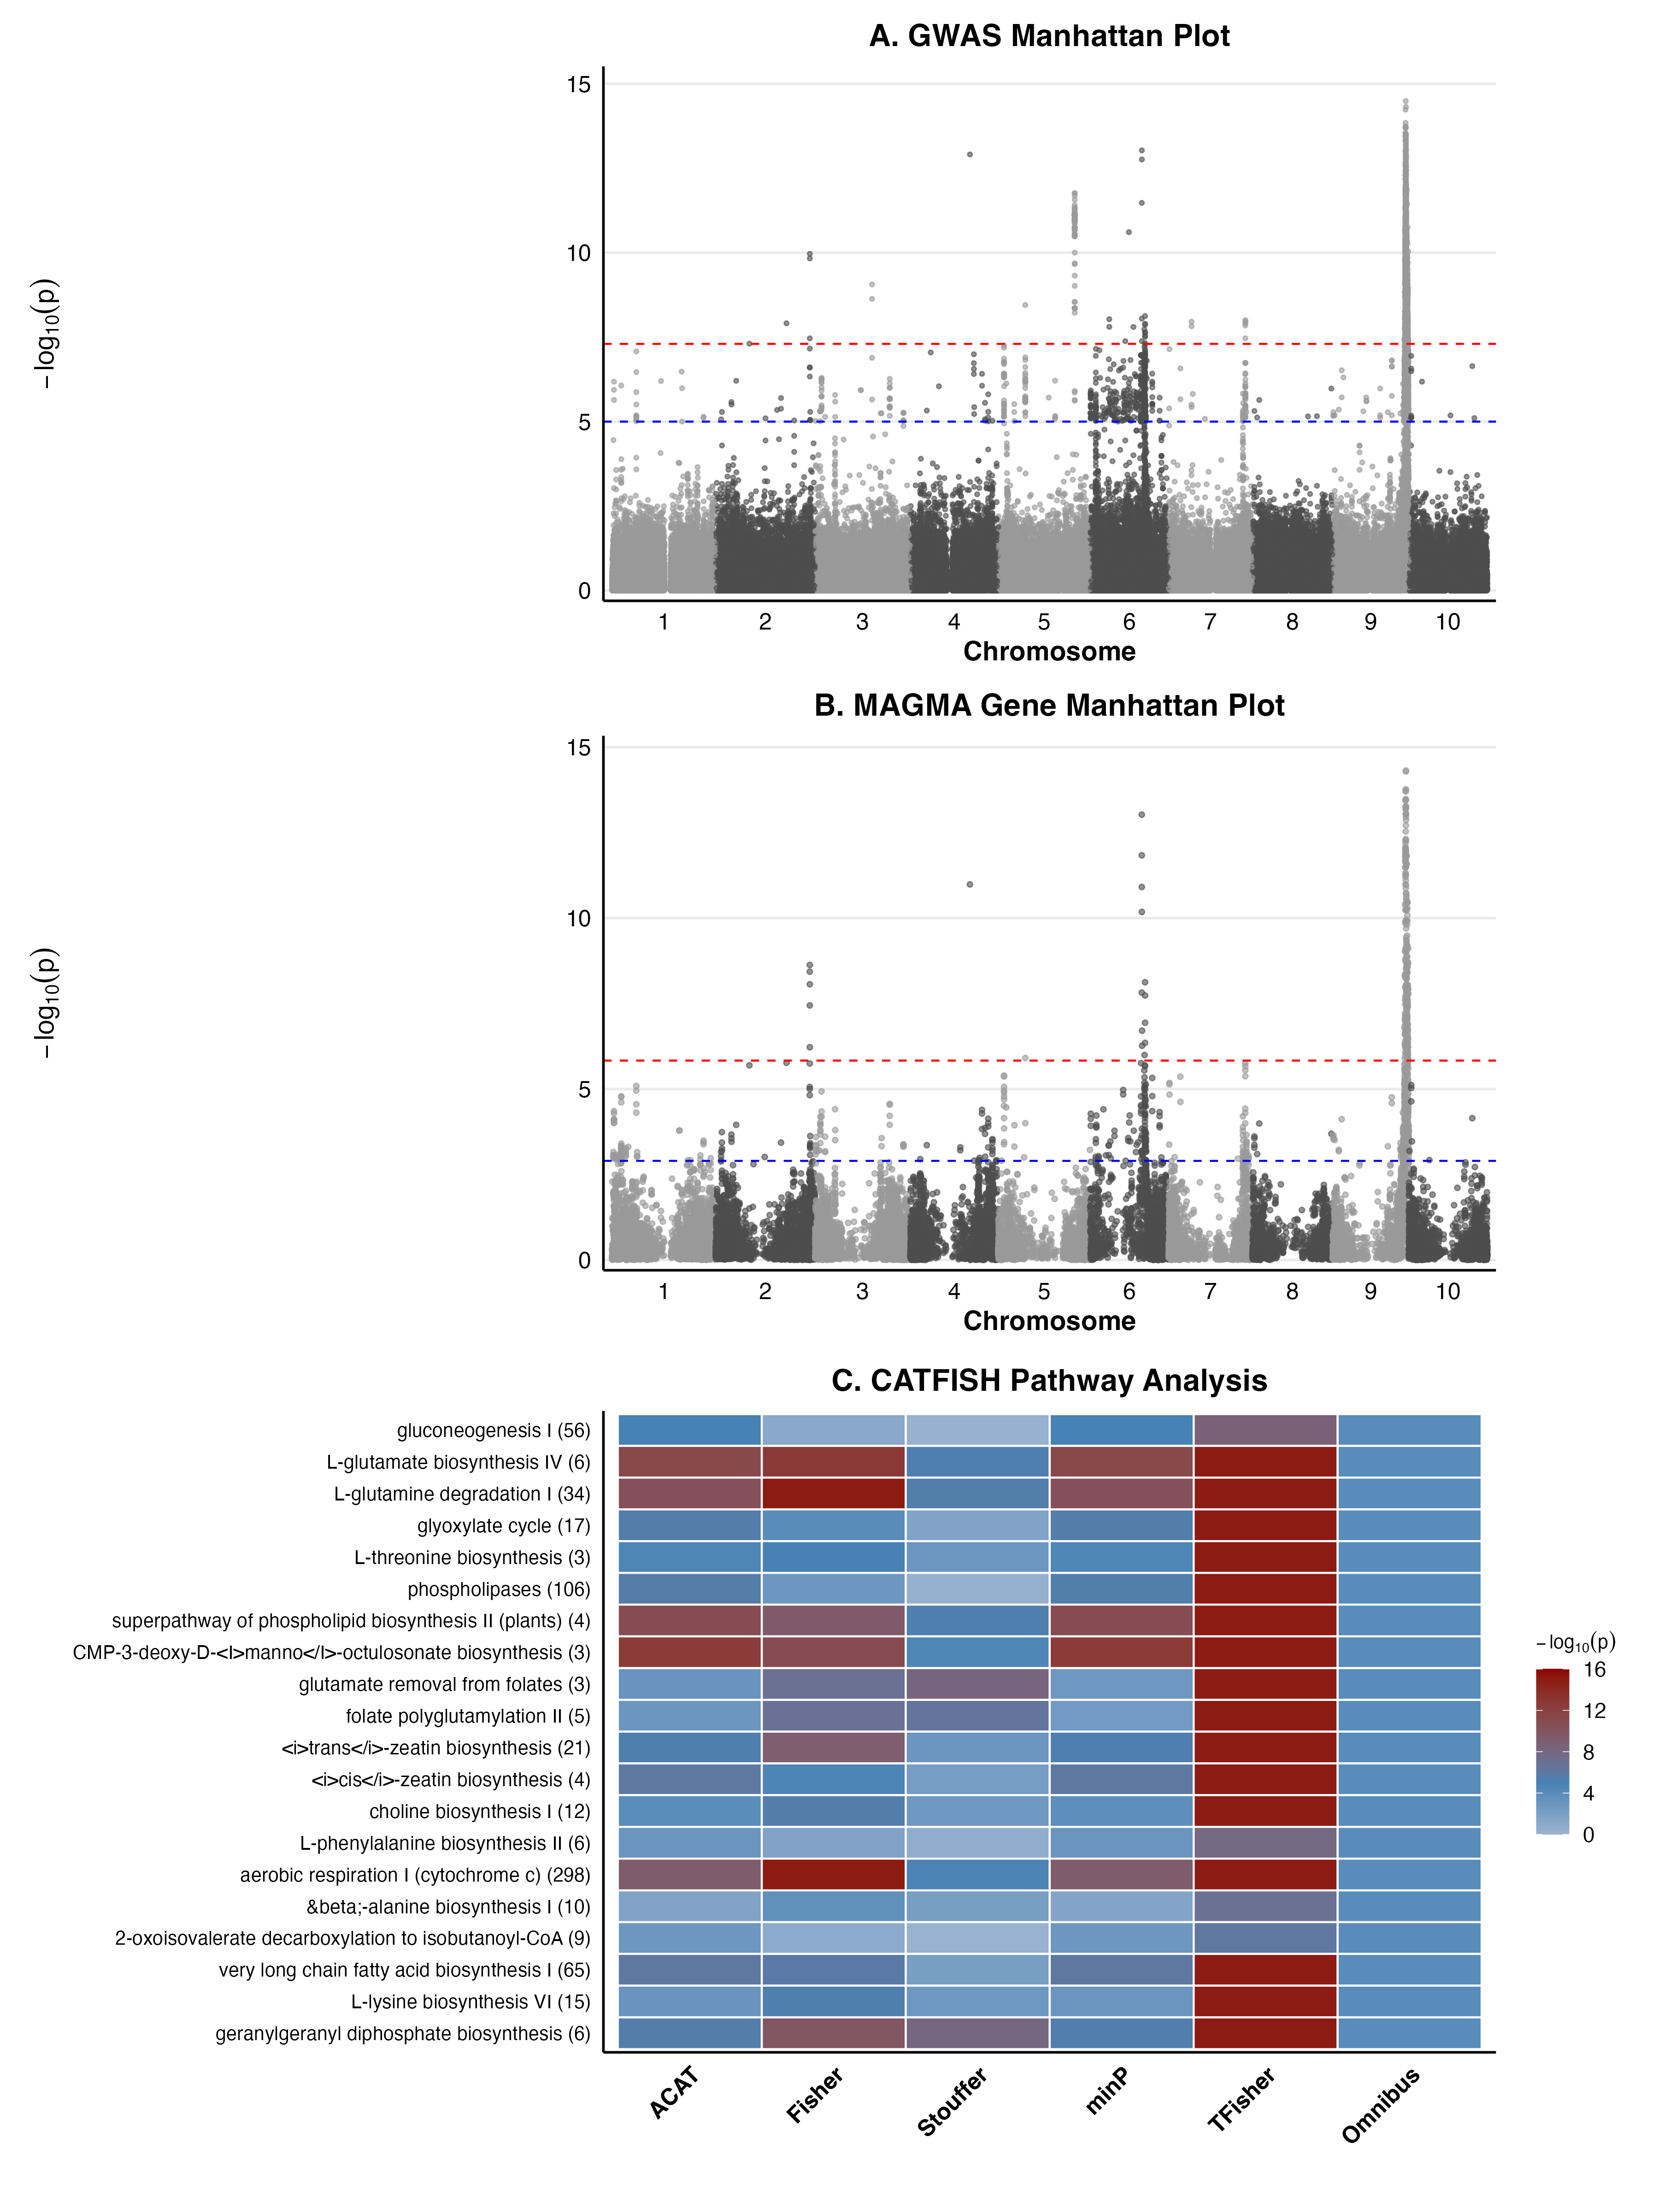
\includegraphics[width=\textwidth]{Figure4_GWAS_MAGMA_Pathway.png}
\caption{\textbf{Genome-wide association and pathway analysis of stem volume in sorghum.}
(A) GWAS Manhattan plot showing SNP associations across 10 chromosomes. Red dashed line indicates genome-wide significance ($p < 5 \times 10^{-8}$); blue dashed line indicates suggestive significance ($p < 10^{-5}$).
(B) MAGMA gene-based Manhattan plot. Red dashed line indicates Bonferroni-corrected significance; blue dashed line indicates FDR $< 0.05$ threshold.
(C) CATFISH pathway analysis heatmap showing $-\log_{10}(p)$ values for top 20 pathways across component tests (ACAT, Fisher, Stouffer, minP, TFisher) and the omnibus test. Numbers in parentheses indicate gene counts per pathway.}
\label{fig:figure4}
\end{figure}

\begin{figure}[htbp]
\centering
% \includegraphics[width=\textwidth]{Figure5_Candidate_Genes.png}
\caption{\textbf{Integrated candidate gene analysis combining GWAS, MAGMA, and pathway evidence.}
(A) UpSet plot showing intersection patterns among genes significant in GWAS ($-\log_{10}(p) > 7$; coral), MAGMA (FDR $< 0.05$; blue), and pathway analysis (Bonferroni $p < 0.05$; green).
(B) Bar chart summarizing gene counts per evidence category.
(C) Density plots comparing $-\log_{10}(p)$ distributions for genes in significant pathways (green) versus other genes (gray), shown separately for GWAS and MAGMA results. Wilcoxon test p-values are indicated.
(D) Scatter plot of GWAS versus MAGMA $-\log_{10}(p)$ values. Points are colored by evidence category; dashed lines indicate significance thresholds. Genes in all three layers are highlighted in red with larger point size.}
\label{fig:figure5}
\end{figure}

\begin{figure}[htbp]
\centering
% 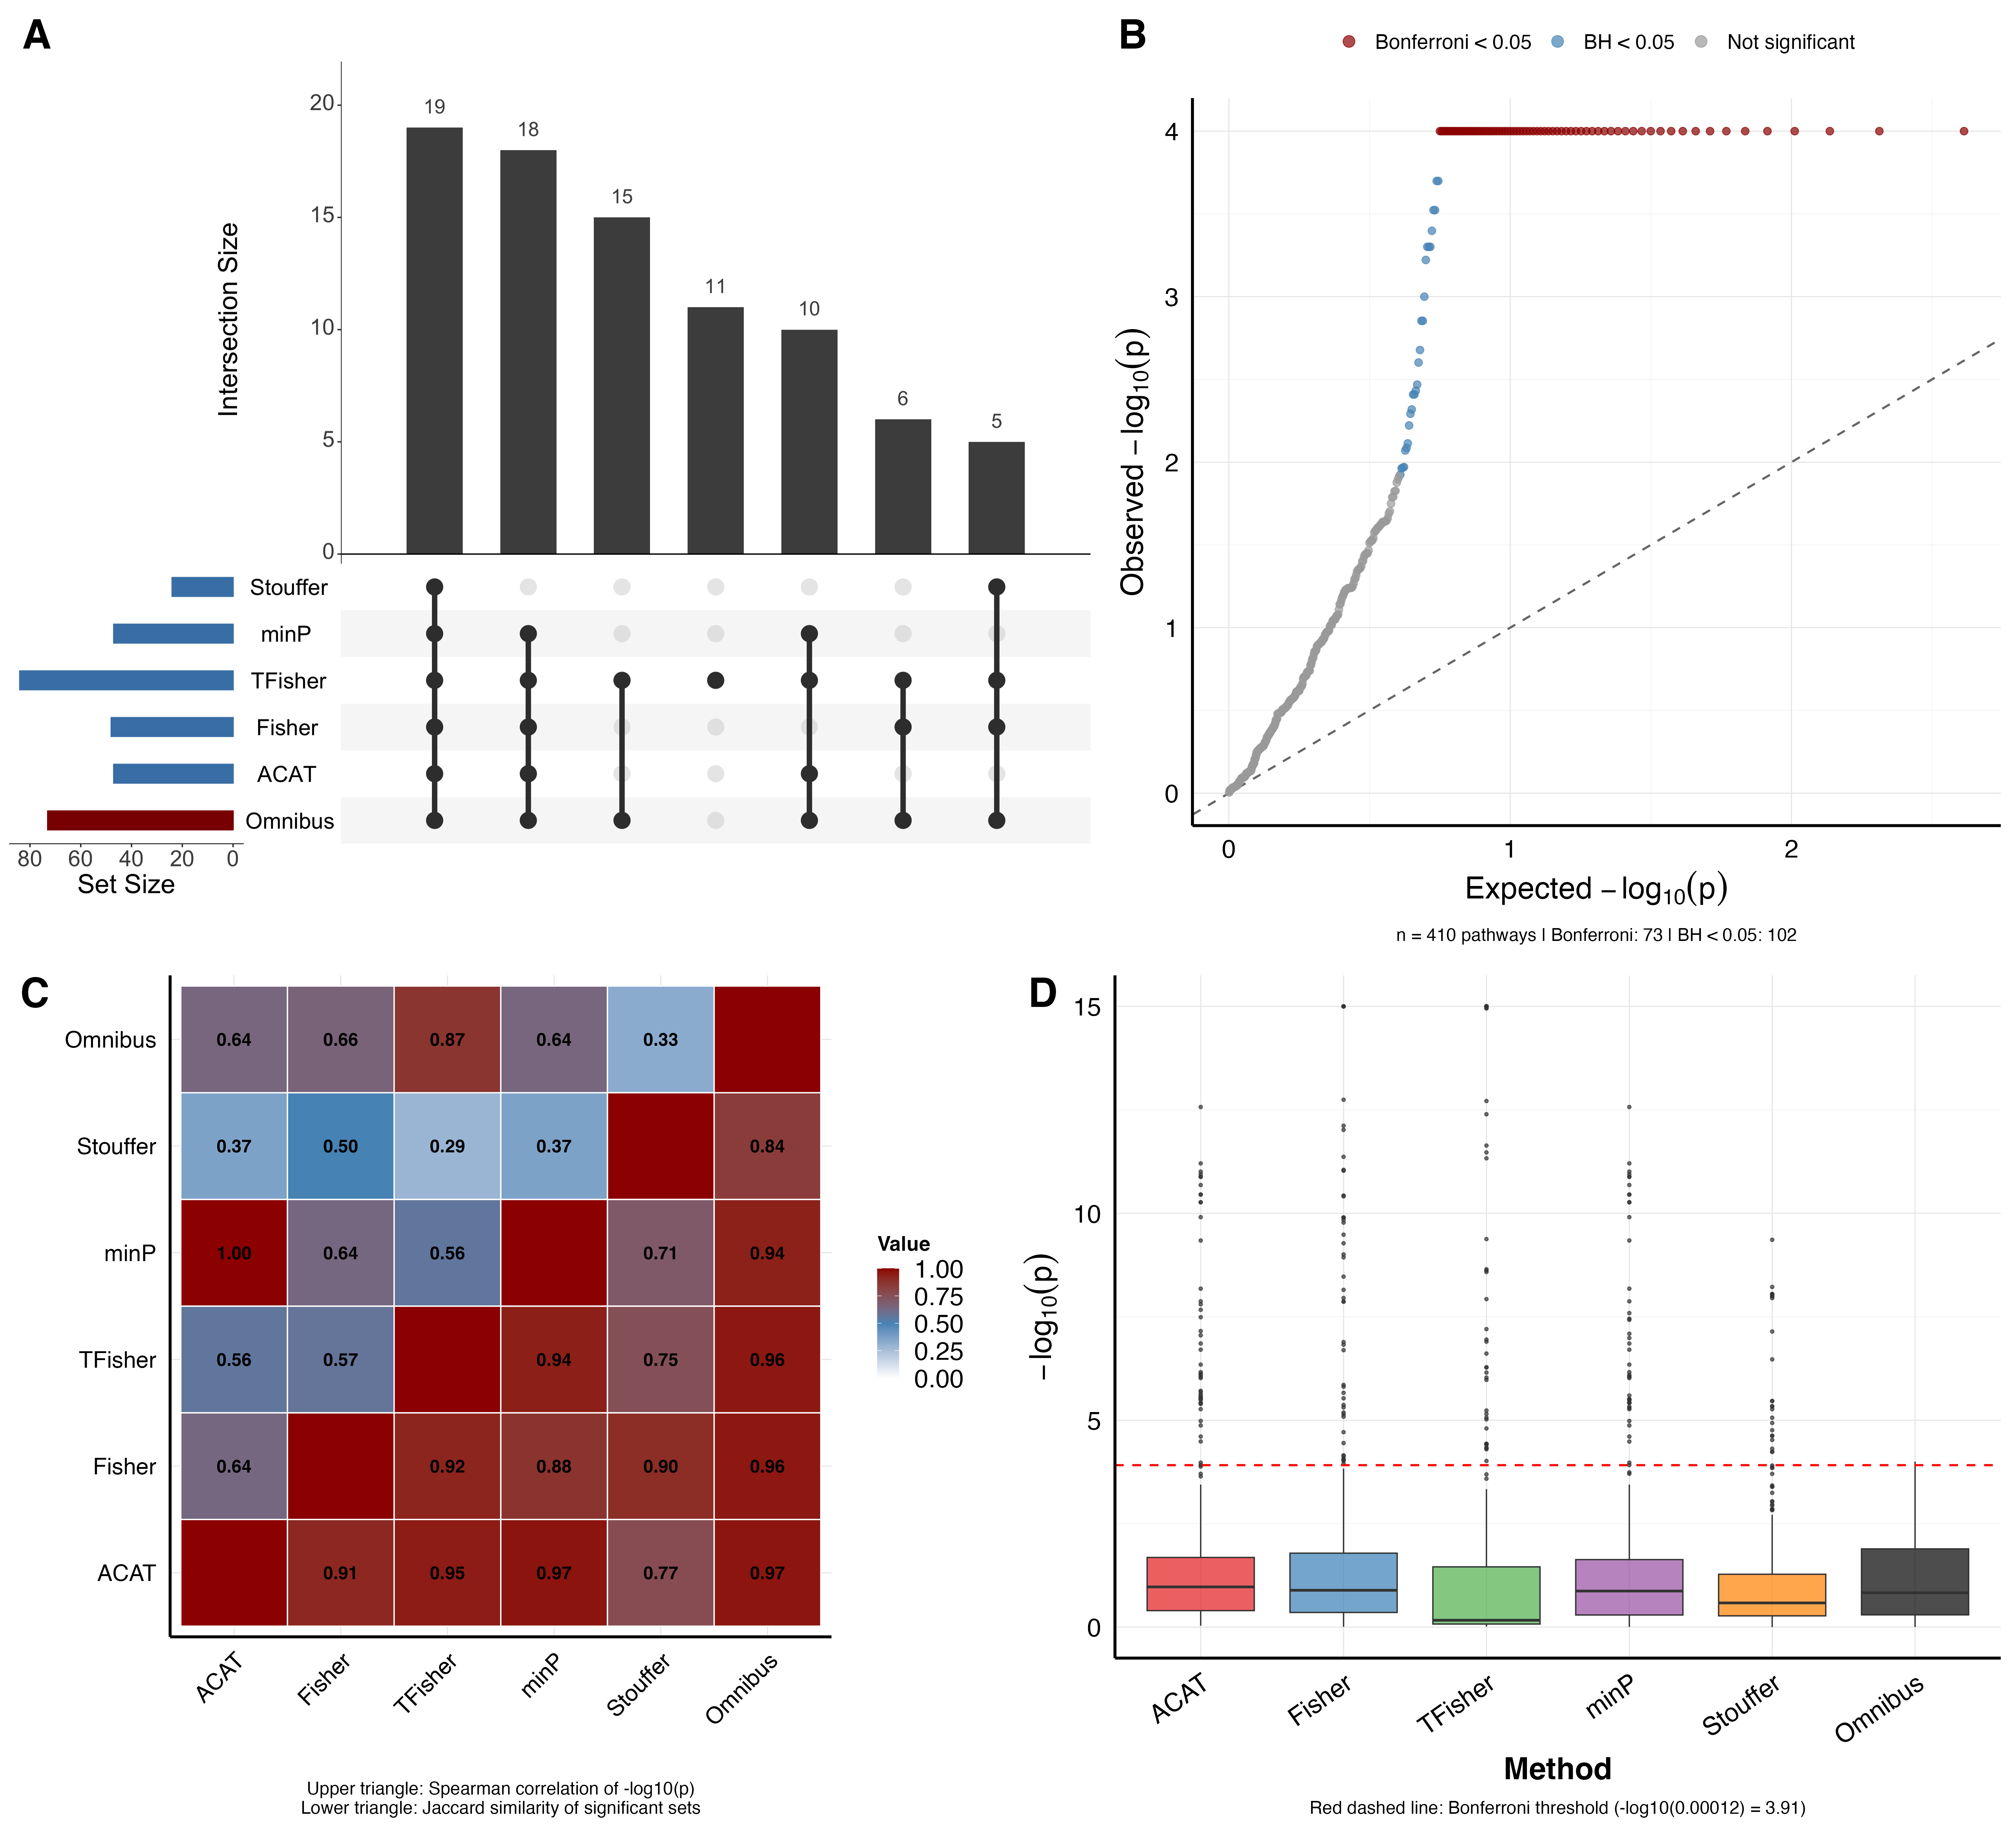
\includegraphics[width=\textwidth]{Supplementary_Figure_Component_Tests.png}
\caption{\textbf{Comparison of CATFISH component tests for pathway enrichment analysis.}
(A) UpSet plot showing intersection patterns among pathways significant (Bonferroni $p < 0.05$) in each component test (ACAT, Fisher, TFisher, minP, Stouffer) and the Omnibus test. Bar heights indicate intersection sizes; horizontal bars indicate total significant pathways per method.
(B) Quantile-quantile (QQ) plot of Omnibus p-values. Points are colored by significance: Bonferroni $< 0.05$ (red), BH FDR $< 0.05$ (blue), not significant (gray). Dashed diagonal represents the null expectation. Non-significant pathways follow the diagonal, indicating proper calibration; significant pathways deviate upward, reflecting true biological enrichment.
(C) Pairwise method comparison matrix. Upper triangle: Spearman correlation of $-\log_{10}(p)$ values. Lower triangle: Jaccard similarity of Bonferroni-significant pathway sets. Color intensity reflects magnitude (0--1 scale).
(D) Boxplots of $-\log_{10}(p)$ distributions for each method. Red dashed line indicates Bonferroni significance threshold ($-\log_{10}(0.05/410) = 3.91$).}
\label{fig:suppfig}
\end{figure}

\end{document}
